% !Mode:: "TeX:UTF-8" 

\BiChapter{绪论}{Introduction of Thesis}

%本章对 \LaTeX{} 排版系统做一个简要介绍,希望没有使用过 \LaTeX{} 的同学对 \LaTeX{} 有一个初步认识。

%=========================================================================================
\BiSection{研究的背景}{What}
\BiSubsection{研究的意义}{Meaning}

%\LaTeX{} 是一款排版软件,和其它排版软件 (例如 Word) 相比,\LaTeX{} 具有非常明显的优势和不足。其最大的优势是高质量、高水准的专业排版效果;最大的缺点是使用门槛高,需要具备一定的编程基础\footnote{因为 \LaTeX{} 的资源非常丰富,有许多模板可以使用,这些模板已经为用户定制好了排版格式,所以单纯从使用的角度看,使用 \LaTeX{} 的门槛其实并不算高。}。对于习惯于抽象思维的科技人员而言,与精美的排版效果相比,\LaTeX{} 的确缺点是微不足道的,只要经过短时间 (一周足已) 的学习和实践,就可以编写出高质量的科研论文。

%\LaTeX{} 的基础是 \TeX,\TeX{} 诞生于 20 世纪 70 年代末到 80 年代初,用来排版高质量的书籍,特别是包含数学公式的书籍。有趣的是,这样一款排版软件并非在排版业界产生,而是由著名计算机科学家 Donald Ervin Knuth (中文名高德纳) 在修订其七卷巨著《计算机程序设计艺术》时设计的。

%虽然 \TeX{} 功能非常强大,但是多达 900 多条的排版命令让排版人员使用起来非常不便。因此 20 世纪 80 年代初,Leslie Lamport 博士给 \TeX{} 编写了一组自定义命令宏包,并取名为 \LaTeX,其中 La 是其姓名的前两个字母。\LaTeX{} 拥有比原来的 \TeX 更为规范的格式命令和一整套预定义的格式,可以让完全不懂排版技术的学者们很容易地将书籍和文稿排版出来。\LaTeX{} 一出,很快风靡全球,在 1994 年 \LaTeXe{} 完善之后,现在已经成为国际上数学、物理、计算机等科技领域专业排版的事实标准,相关专业的学术期刊也都采用 \LaTeX{} 作为投稿格式。

21世纪的新20年,网络正以前所未有的速度越来越紧密地参与到民生社会中,对满足国家民生需求、新基建拉动内需和产业升级起到了至关重要的作用。从“百度一下”到网红全民直播带货,从实现“三网通”到发展“新基建”的国家战略,小到优化社会资源效率的办公数字化,大到勾勒出智能交通、智慧城市和万物互联的5G海洋,无一不是构建在网络基础设施的快速发展之上。思科公司预计,到2023年全球家用互联网总带宽将达到$5.85Ebps$\footnote{$1 Ebps=10^6Tbps=10^{18}bps$} (是现在的3.27倍),移动互联网用户预计达到57亿,其总流量可达$11.3Ebps$ (将达到目前的5倍),其中5G流量将占据移动互联网总带宽的76.5\%(0.6\%,2019年)\cite{huawei2019,cisco2019}。由于深度学习、AI、大数据、云计算、物联网的快速发展,这些新技术将催使新零售、新金融、新医疗、新教育、新制造、云视频和云游戏等行业“云化”,海量的数据会在数据中心内部服务器间网络中及对外网关中交互,这些关键应用将会改变数据中心算力和数据中心内部网络结构特性。

IDC报告称,2019上半年中国公有云服务整体市场(Iaas/PaaS/SaaS)达到54.2亿美元,并预计在未来5年间内以年均复合46\%的速度快速增长\cite{idc2019,idc2020}。数据中心内服务器计算力呈现异构化趋势,GPU, AI Chip, FPGA等使用非通用类型指令集和特殊体系架构计算单元已成为目前分布式计算领域的热点话题。现在超大型数据中心一般可容纳数十万台终端服务器,内部网络链接数量多、拓扑规模大、传送海量数据,这使得现有的网络将变的异常复杂。同时,新的数据包类型层出不穷也使得现有网络变得异常脆弱。

传统网络技术已经无法满足当前的网络环境的需求,最近十年来网络技术和架构经历了快速地演进和变革,针对数据中心网络尤为明显。传统网络的互连包含了经典的二三层网络。为增强交换机的扩展能力,二层网络增加了广播,桥接等复杂功能。这种网络架构在小规模应用时可以展现强大的智能性与可扩展性,但当网络规模进一步增加,网络中容易出现的广播风暴、链路收敛等一系列尖锐问题变得难以解决。现代的大型网络设计思想摒除了略显冗余看似小聪明的功能设计,事先规划好网络拓扑层次,完整地保留网络的第三层,从而将网络扁平化。网络拓扑结构演化出可进行大规模扩展的CLOS型架构,为了降低系统复杂性,在各个层次之间的网络设备功能也逐步变得统一透明。网络设备统一化,可降低网络功能开发部署的难度。通常,研究人员需要持续地投入对网络进行测量、监控、容错、提升效能的工作。由于思想的创新和技术的推进,设备厂商不断开发出具备各种高级功能交换芯片。设备、芯片功能强大的同时,复杂的网络功能不断地对于网络的管理层又提出了新的挑战。

为解决设备制造复杂和设备管理复杂的问题,软件定义网络(Software Defined Network,SDN)概念的提出拨开了笼罩在网络体系结构发展道路上的迷雾。SDN将数据平面和控制平面解耦。在数据平面上,对数据包的处理统一做查找-转发(Match-Action)抽象。控制平面复杂建立网络拓扑,控制并下发流表。这样所有的数据包转发行为都又控制平面的软件逻辑完成,数据平面可以支持任意一种网络协议的处理。由于软件具有强大的灵活性以及开发的敏捷性,SDN大大加速了网络创新和智能化进程。数据平面和控制平面的安全通道由OpenFlow协议进行规范,将数据平面统一化、简单化,使得网络交换设备向白盒化方向发展。

大规模网络无论是在底层设备架构还是运维方式上仍不能停止变革的脚步,这为可编程硬件的发展带来了巨大空间。随着云服务概念和大规模机器学习的落地,近年来以云计算为代表的数据中心网络规模指数增长。网络功能虚拟化在数据中心内部是关键一环。虚拟交换机则是主机内各虚拟机之间数据包转发的核心软件。随着众核CPU架构快速发展,服务器内虚拟机布置资源大幅扩张,促使主机出口吞吐量从40GbE向100GbE甚至400GbE演进。不但如此,复杂的网络安全规则、流量监控等模组进一步导致CPU过多地消耗在处理网络功能上面。研究人员可能需要花费大量时间去解决目前网络架构的大规模扩展的方案。(创新变的异常艰难)。传统x86CPU架构适合于处理灵活多变的计算控制任务,对于做重复、常规流式数据处理,通用指令集架构并不能得到最优的效率,厂商往往不得不依靠大量部署server来解决。为缓解主机内CPU消耗过大,目前提出的智能网卡是一种新思路。智能网卡采用FPGA,网络处理器,ARM等器件,或以他们的组合形式形成在网卡端的新的算力集合,这种算力集合对于处理网络流量会有更高的效率。我们可以把转发动作,网络安全规则等功能下放进来,以削减服务器CPU的额外消耗。ASIC具有最好的性能和最高的能量效率,但每次大批量的部署消耗时间长,投入研发资金大。对于运营商来说,设备、仪器等一次性支出都叫做CapEx(Capital Expenditure,资本性支出)。对于目前快速发展的网络环境架构,设备的更新换代周期也在变短,在优化CapEx时已经不能把固定设备投入当做一次性支出。在探索新一代网络架构时,CapEx也会成为重要的参考因素。

随着创新性和需求的进一步发展,让底层硬件拥有灵活的可控制能力才能满足目前行业变革的需求。因此,网络领域提出了编程协议无关(Programming Protocol-Independent Packet Processors,P4)概念。P4协议不但支持SDN网络控制和管理的可编程性,还提出了数据平面可编程的概念。数据包在数据平面内的处理模型遵循解析-查找-匹配的抽象模式。P4规定了一种编程语言\cite{p4},它可以控制数据平面对数据包的任意解析行为,也可以自由配置查找表的数据位宽和多级流表之间的查找流水线\cite{rmt,mswitch}。这种更高阶的数据平面可编程模型使交换机设备更加白盒化,交换机与任意网络协议解绑,带来了具备灵活性的创新实践。除此之外,端到端大带宽、低时延的网络需求引申出了网络功能硬件卸载、网络随路计算等概念,这进一步增强了对高性能的网络数据平面可编程性的需求。

综上所述,现代网络在向软件定义、数据平面可编程的方向发展。网络架构的变迁的核心是有一套可以映射上层可编程逻辑的硬件数据平面。本文主要探索一种面向网络数据平面的可编程硬件,能够满足快速迭代的网络创新性需求,同时能够提供与目前主流设备相仿的处理性能,以及可扩展性高的全局优化方法。

\BiSubsection{技术简介}{shortintro}

软件定义网络的基本设计概念是将数据平面与控制平面分离\cite{mckeown2008openflow,ethane}。其中,网络数据平面是指完成计算机之间通信数据包的匹配、修改、传送、转发的软硬件设备。数据平面的可编程性要求网络管理员拥有对数据平面的各个特性做快速个性化定制。网络的控制平面维护全网视野数据,配置针对流的转发条目,控制平面中的应用程序几乎都由软件构成。当前数据平面的设计思想如图\ref{sdnarcs}所示,主要有软件方法实现,专用硬件实现和新设计的可编程硬件。

\begin{figure}[!ht]
	\centering
	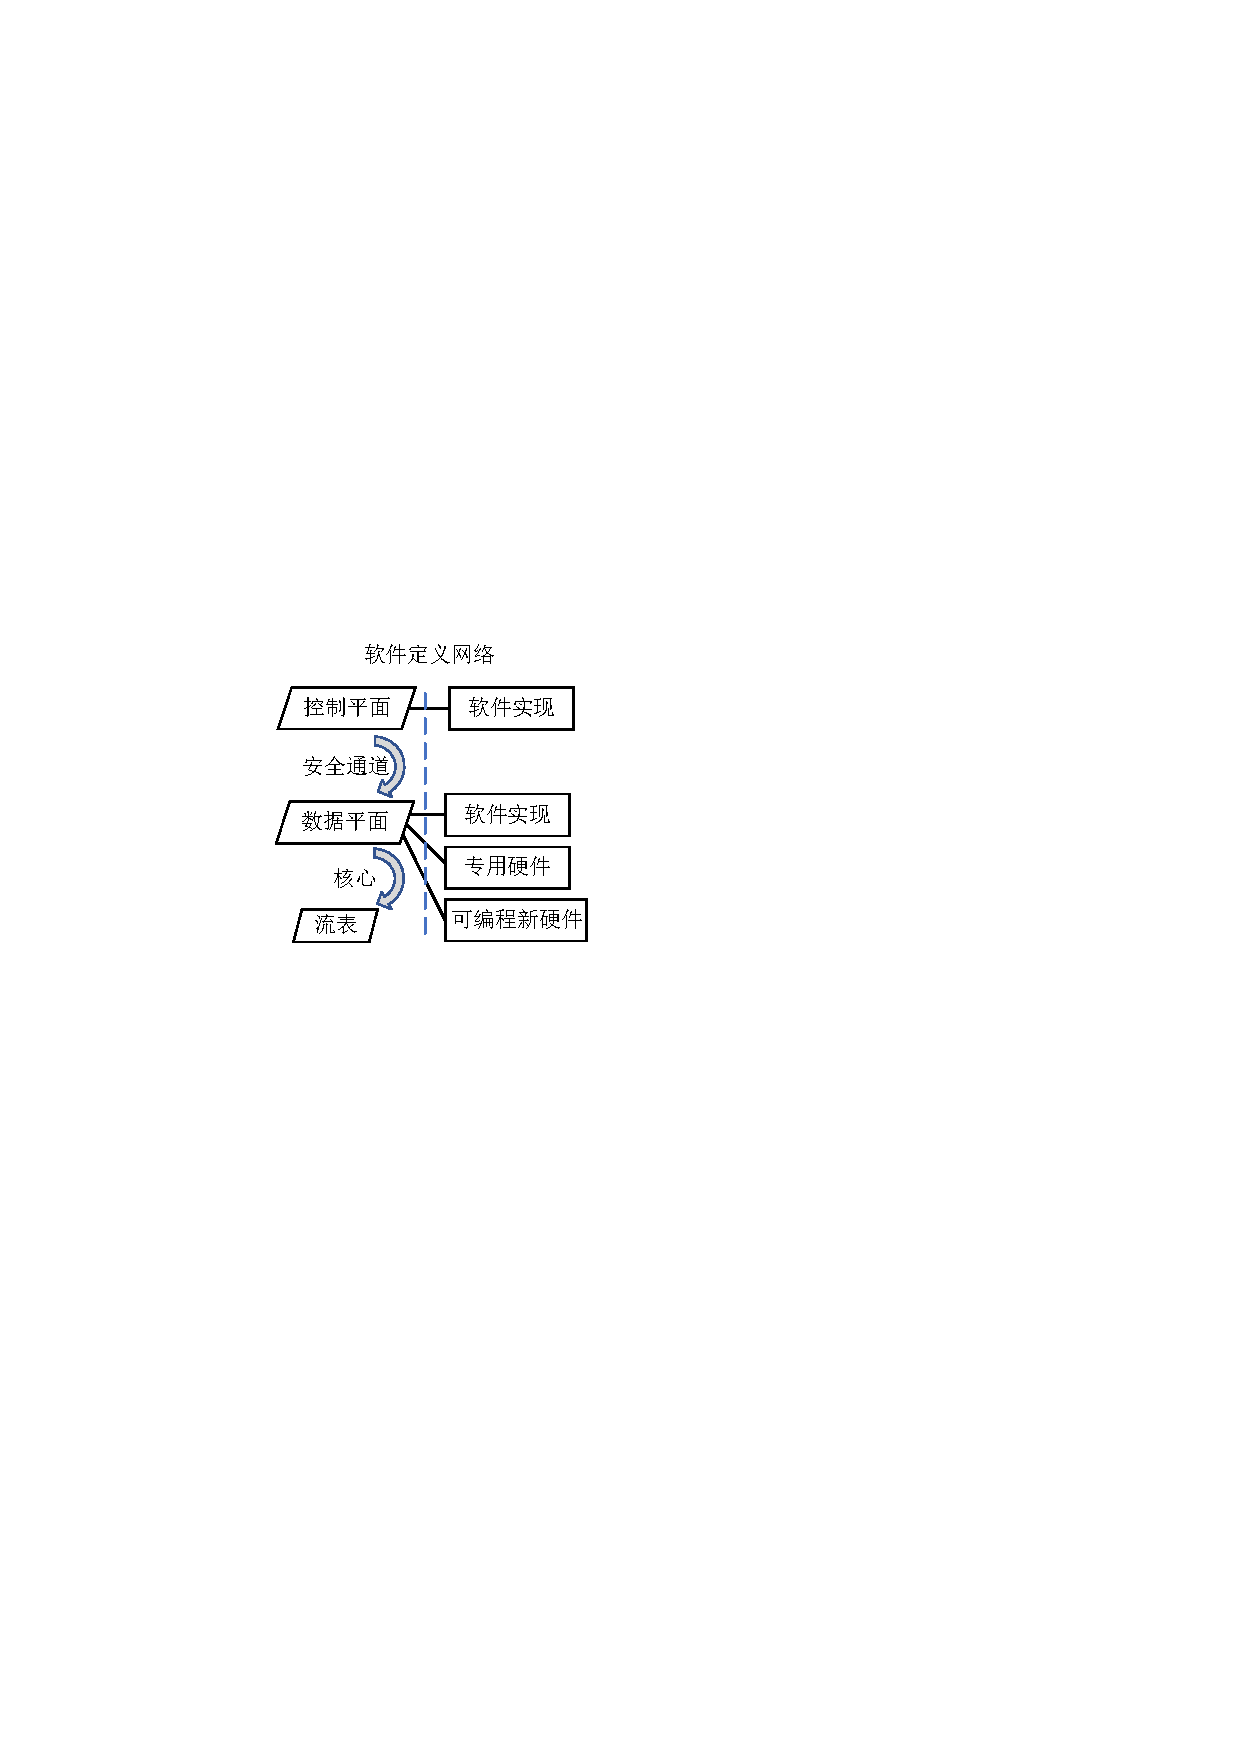
\includegraphics[scale=1]{sdnarcs.pdf}
	\caption{软件定义网络结构及其实现方案} \label{sdnarcs}
\end{figure}

在不同场景下,网络对于数据平面的需求千差万别,研究人员一般根据场景的流量大小,处理过程复杂度来思考并选取数据平面的实现方案,本文将在第\ref{sec:pdpintro}章详细介绍各类数据平面的实现方案的优缺点,并着重于可编程性的分析。目前两种最重要的数据平面是“软件交换机”和“专用硬件交换机”。两者在功能上都是针对数据包做一系列处理,包括匹配、查找、统计、传送、转发和安全校验等等,其中“流表”是实现数据平面核心功能的函数(器件)。数据平面、都包含一个可以与远端控制器沟通的软件代理,这部分功能着重于通信协议的实现以及通道安全性加解密,主要由轻量级通用处理器完成。其二者的主要区别在于处理数据包的性能以及交换容量。数据包处理性能主要看数据吞吐量(字节每秒)和包吞吐量(包每秒),目前软件交换机做高性能的包转发几乎可以达到60G/60Mpps\cite{pisces}。当数据包处理复杂度增加时,软件交换机的性能会直线下降,几乎与操作步骤数成反比。专用硬件交换机有接口数目多,交换容量大的特点,一般能满足64口乘以每口$25Gbps$的总交换容量。而且硬件交换机的性能与数据包处理步骤几乎无关,它拥有良好的性能稳定性,低转发时延等特性。虽然在核心网络和高性能网关领域主要使用硬件交换机,但是硬件交换机的功能固定,更换成本高昂,如果需要修改网络或者更改网络功能那么选用专用硬件交换机的场景将无从下手。所以目前在数据中心网络或服务器NFV(网络功能虚拟化)等场景中,软件交换机依然占据很大份额。由于软件交换机的灵活性高,开发人员能够快速迭代部署新功能,且传统单机CPU通信速率需求不高,软件交换机尚能满足在数据处理时延高、吞吐率低的前提下,提供足够的可编程灵活性。但随着人工智能领域、5G的发展,数据中心网络内通信容量需求快速增长,转发时延需求快速收紧,软件交换机性能瓶颈快速到来,将不得不面对大量无谓堆叠CPU的情形。本文将主要侧重于研究主机侧网络和核心交换网络中使用可编程硬件来大大提高交换机的性能瓶颈。针对控制平面,本文将从单点优化开始用分布式优化和全局优化的思想,实现对网络中的瓶颈资源(如流表资源)的可扩展性和安全性提升。

\BiSubsection{国内外应用与研究现状}{inoutintro}

为增强数据平面的可编程性,工业界学术界互相促进、广泛研究并已经提出了许多方案。

1)基于软件的数据平面

这类技术着重于开发便捷,价格低廉,无需在网络中部署专用设备场景,是快速实现功能的首选方案。目前在虚拟化的云服务系统中,已经部署了大量基于软件的功能:a)转发层,华为CE1800V\cite{huawei1800v}是专为数据中心云计算虚拟化环境部署的一种分布式虚拟交换机。其支持标准Open Flow1.3控制协议,以及Open vSwitch 数据库管理协议(OVSDB),基于英特尔DPDK(Data Plane Development Kit)技术提供每核12Gbps的转发吞吐,比业界平均水平高出20\%。b)流量监管,Activelogic\cite{activelogic}是一个提供安全可靠、流量分类、提高QoE(Quality of Experience)能力的网络管理工具。它基于软件可自动化部署,依靠超大规模性能、人工智能技术以及云计算场景优化的能力,在数据平面解决流量监管的问题。基于软件的数据平面功能可以依靠堆叠CPU核数来实现大规模的性能扩展,但由于计算复杂度过高、基于指令的图灵机在高速内存共享和海量数据处理场景中效率低下,即使简单转发的性能达到100Gbps线速也需要占用8个核心以上\cite{pisces,v580}。综上所述,我们发现单纯地依靠软件处理器扩张来增加网络性能边界收益将越来越小。

2)基于白盒交换机和P4专用芯片的数据平面

在网络性能方面大幅超越基于通用服务器的NFV数据平面\cite{p4,v580}。符合OpenFlow规范的白盒交换机可将控制平面移交给远端软件层,从而大幅提升设备的再开发能力,在DDoS防护、负载均衡等基础网络转发设备的智能化和可定制化方面给出了比较好的灵活性。阿里巴巴在其云计算网络场景中,通过可编程硬件交换机和通用服务器结合来实现公有云的网关服务。此架构既享受到芯片带来的网络转发性能提高(6.4Tbps,400ns延迟)和可编程能力带来的网络功能快速部署迭代,又能实现软件所擅长的复杂网络调度功能\cite{alibaba}。这样同时兼顾了性能、灵活性,在大规模扩展网络体系结构时达到降低成本,满足业务需求和简化网络架构同时提升服务稳定性。数据平面可编程芯片提供了硬件层面上的可编程包头抽取器、可编程流表以及可编程执行器,他们的设计思想是依靠快速查表(TCAM,SRAM)法,或经过后期编程选取特定的冗余逻辑模块(在ASIC芯片内部的空间上堆叠的可编程单元)法,来完成专用电路(ASIC)的直接描述逻辑\cite{rmt,tofino2}。不过这类可编程芯片架构提供的可编程执行器是不完备的,前后堆叠的流表限制了流表的宽度、深度范围,会造成逻辑资源浪费以及流水线处理延迟过长。同时,ASIC设计定型之后无法增加新的用户特性(状态转发、随路计算、监测计数和包调度特性),导致这类P4专用芯片的可编程性是大大受限的。

3)基于FPGA的自主设计的数据平面

现场可编程门阵列(FPGA)是一种灵活性可以与软件媲美可编程硬件,性能和效率与专用硬件比较接近。现代高速度云架构依赖于每个专用硬件(ASIC)网络节点的支持,随着网络功能需求多变与复杂化,ASIC类型的网络处理芯片已经不能提供足够的可编程性,然而CPU核心无法提供高的处理性能。业界已经开始将网络堆栈向基于FPGA的自研网卡中卸载\cite{serverswitch,azure}。为了推广可编程硬件,学术界牵头推出了基于FPGA的智能网卡开源项目NetFPGA\cite{netfpga2014},业界龙头企业Xlinx、Intel等也纷纷推出了基于MPSoC/FPGA的自适应计算加速平台Alveo\cite{xilinx,alveo}系列智能网卡和N3000\cite{intelfpganic}。目前,基于FPGA的可编程数据平面已经广泛应用在5G接入边缘网络\cite{intel5g}、数据中心计算存储\cite{xilinxnvme}、核心网络低延迟加速器\cite{intelgre}以及高性能高可靠性高安全性的数据中心防火墙\cite{intelddos}加密通信\cite{intelencryption}等领域。FPGA的高灵活性由全可编程的逻辑门带来,目前一般用硬件描述语言Verilog、VHDL等开发。一个合格的硬件工程师的培养周期要远大于软件工程师,这也是目前网络领域硬件卸载最难所在。为了解决这种不足业界也推出了一系列类似C语言的高层次综合工具HLS\cite{xilinxhls},但使用这类工具必须学习1000多页的开发文档\cite{hlsdoc}。并不是所有代码都可以直接被工具转译,而且还需要考虑到硬件细节,降低FPGA资源消耗;需要自主决定并行区块;需要在代码中融入这种编译器的特性标记字符,总体来看,目前并没有从本质上改善对硬件编程的困难程度。除此之外,由于在FPGA中复杂逻辑对并行总线宽度的时延敏感度高,一个大型工程的主频一般不会超过200MHz,即使每个时钟节拍都可以处理一个数据包,那么FPGA流水线在处理最小包时的最高吞吐量也只有134Gbps\footnote{134Gbps=200Mpps*(64+20)*8bits},这对进一步需求性能的核心网包交换场景也形成了瓶颈。

\BiSection{研究内容}{is}

本文主要探索基于可编程硬件的高性能网络数据平面。论文提出基于可编程硬件的网络数据平面,对主机侧网络和交换层网络的数据平面实现加速,并研究在软件定义网络(SDN)概念下控制平面对全网核心流表资源的全局优化方法。如图\ref{proghardwarePDParcs}所示,论文把操作系统软件网络堆栈的大负载的网络存储和计算功能向网卡硬件卸载,利用FPGA与交换芯片使能交换网络数据平面的高性能高可编程性,把数据平面的主机侧网络、交换层网络的普通转发设备替换为具有硬件可编程特性的网络设备。流表资源是网络转发数据包的核心指令依据,本文基于软件定义网络控制面数据面分离的特点,对全网的流表资源进行了全局效率、可扩展性和安全性优化。

\begin{figure}[!ht]
	\centering
	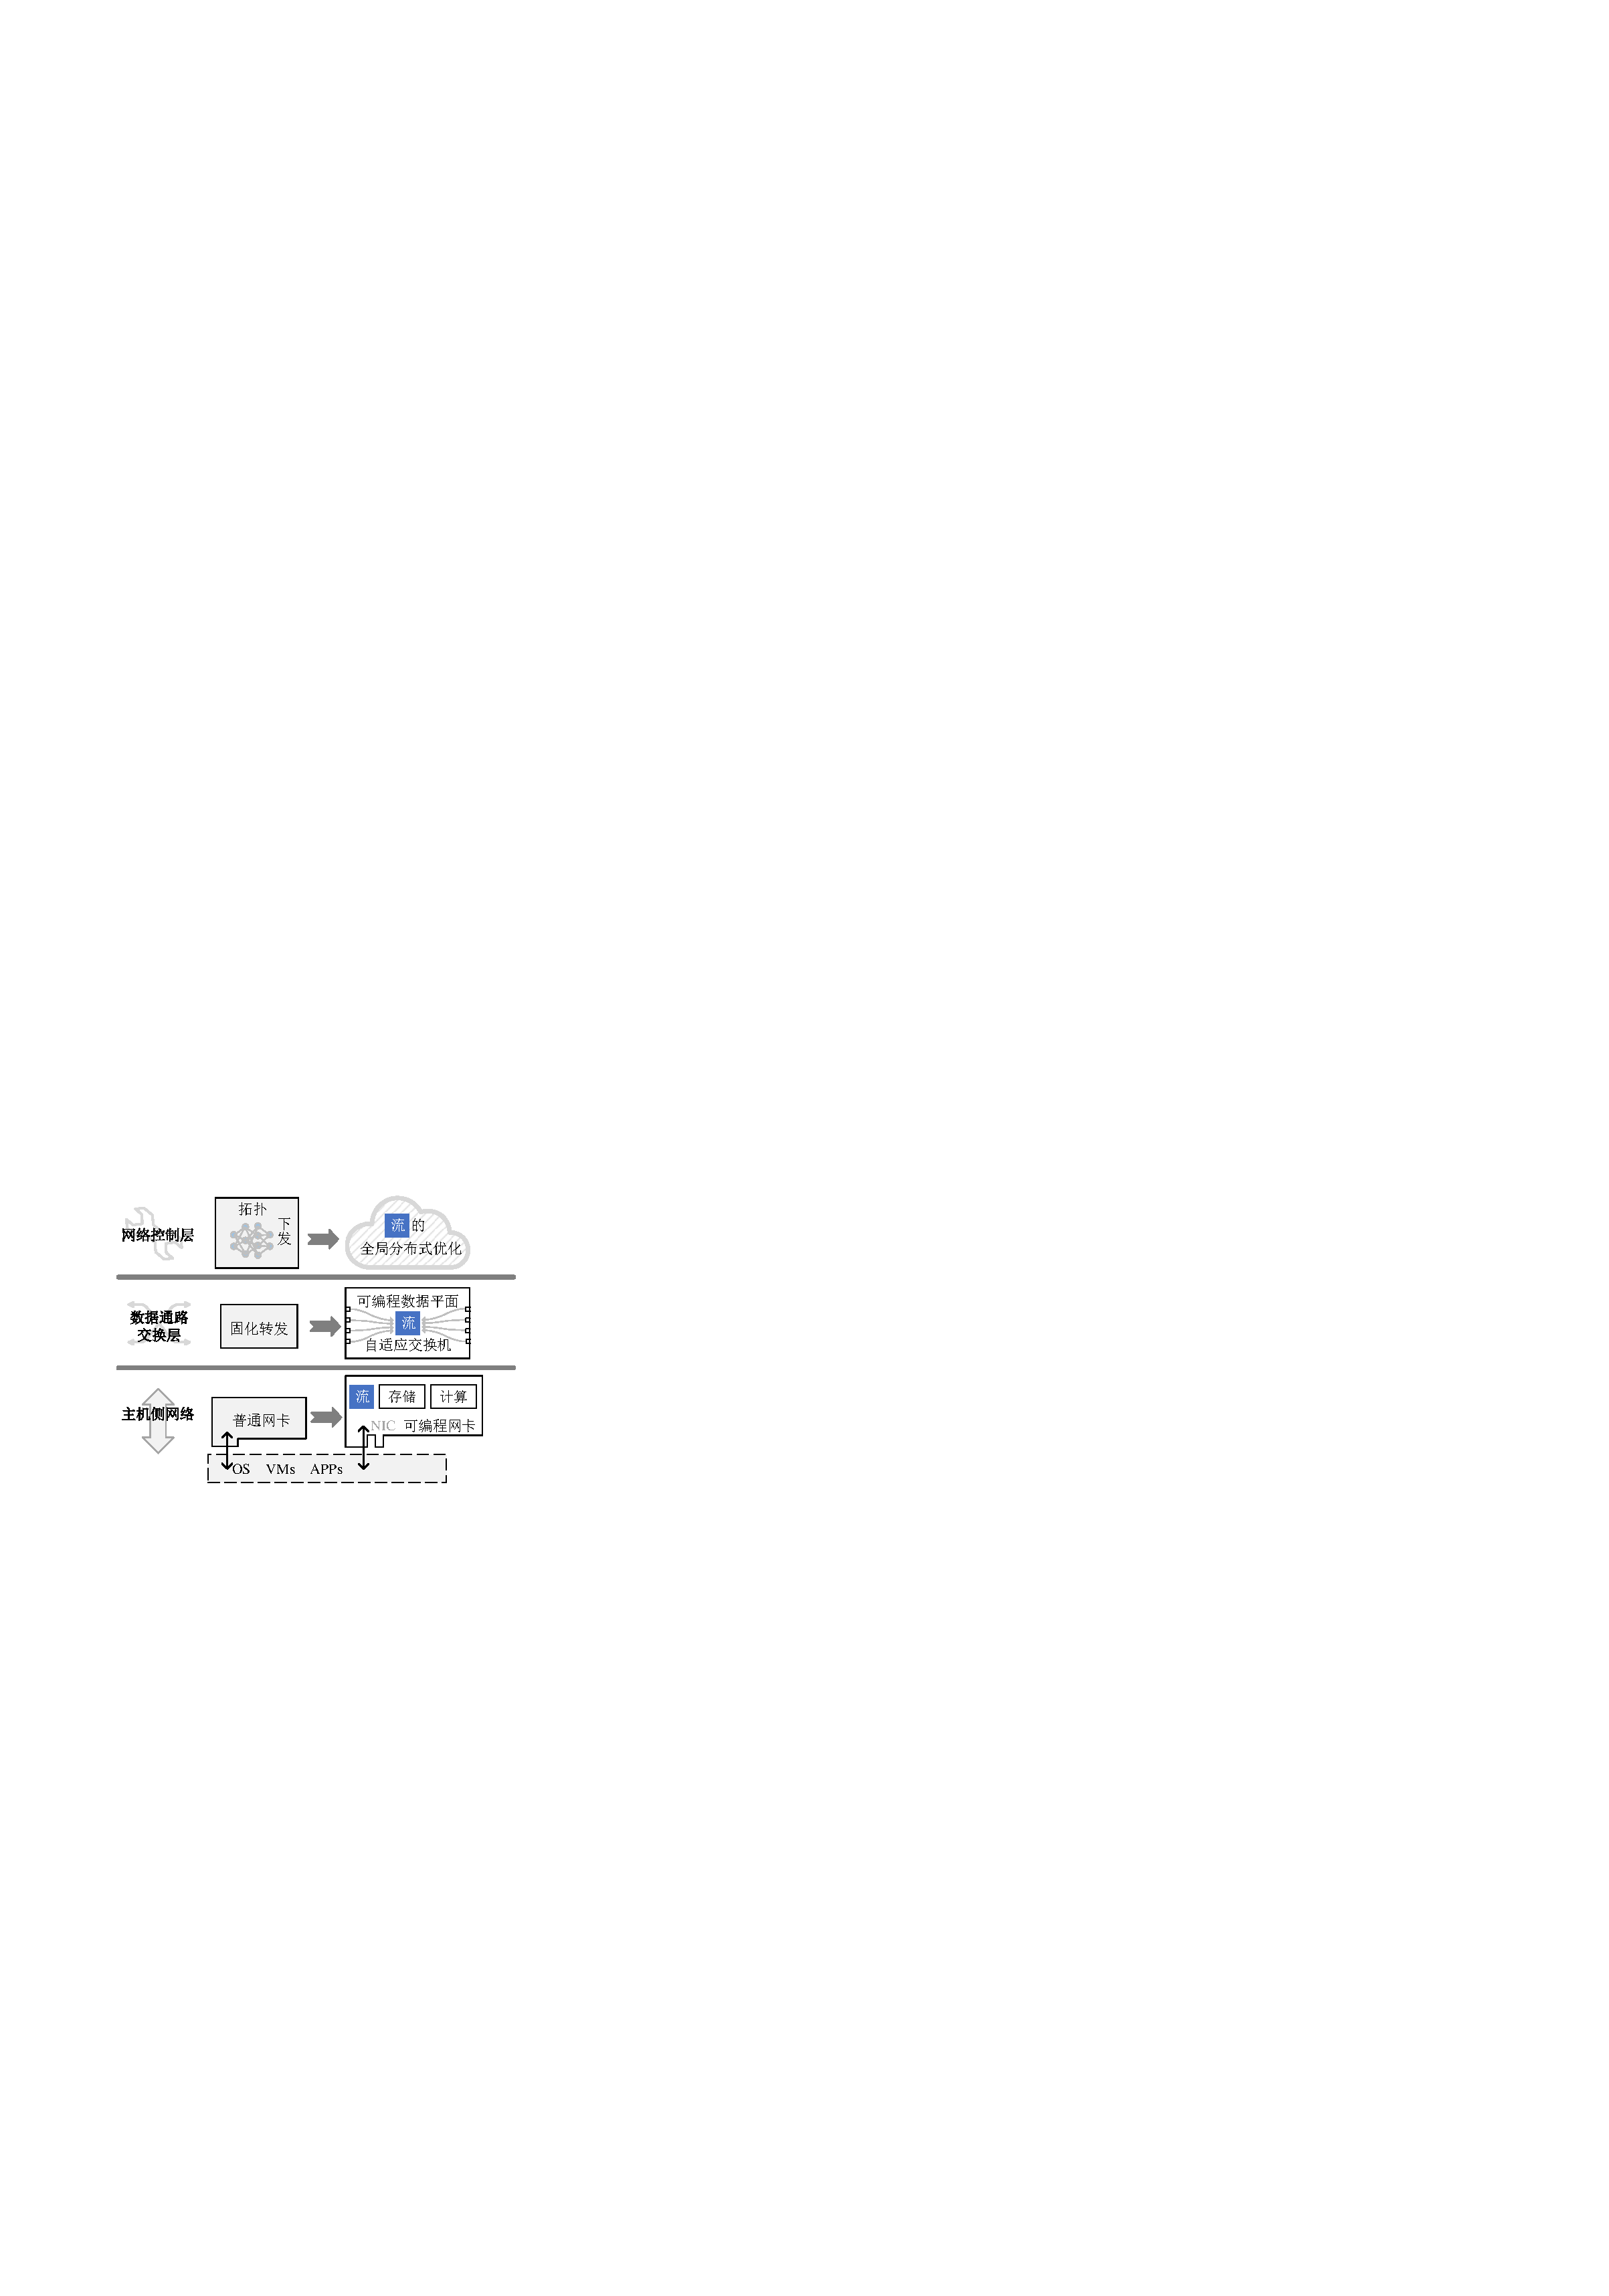
\includegraphics[scale=1]{proghardwarePDParcs.pdf}
	\caption{基于可编程硬件的SDN数据平面研究框架} \label{proghardwarePDParcs}
\end{figure}

1)研究可编程设备加速主机侧网络方法

本文提出利用基于FPGA的智能网卡卸载操作系统层部分网络功能,以达到扩展网络接入层的性能的目的。探讨了不同场景下网络功能的构成,分析并提出一种基于可编程硬件的网络功能定义抽象(Data-Computing,DC抽象)。本文把服务器网络功能任务中可转化为DC抽象的计算密集型功能通过合理转换下放到网卡的FPGA可编程器件中。论文针对网络流量捕获,统计分析和回放等功能场景,将其功能利用DC抽象方法,合理化地卸载到硬件网卡。在满足网络功能不受改变的前提下,证明利用基于FPGA的智能网卡能有效地提升服务器的网络性能、时延和效率。

2)研究可编程设备加速网络硬件交换层方法

本文提出一种硬件异构型的可编程网络数据平面架构,将FPGA与ASIC交换芯片有机结合,以增强ASIC报文处理报文的灵活性,同时满足性能需求。论文设计了ASIC面向硬件可编程扩展的接口,将数据包头拆分并通过高速数据互联载体发送给FPGA,利用FPGA可重配特性实现完全可编程的报文处理数据平面;同时,本文基于DC抽象,将网络随路计算(network-centric computing)模式引入可编程网络体系架构;本文通过分析流量模型在FPGA中设计了一种并行化处理单元,在资源消耗可控的前提下大规模提高系统的可扩展性能;另外本文提出了一套基于可编程硬件混合网络架构的软件定义语言编程框架,实现了软件定义需求和可编程硬抽象层分离,以及针对底层数据平面的一种高效自适应的并行单元流分配算法,可以稳定实时地保障系统交换层的高性能。

3)SDN硬件流表可扩展性研究

本文针对不同层面网络设备的控制,进行全局优化、分布式优化。在可编程网卡和交换机组成的网络系统中,数据平面内最重要的资源是流表资源(瓶颈资源),本文从全局视野角度,结合可编程硬件的特性,在全网约束的条件下,对流表资源进行优化,以满足未来可扩展性需求。本文分析不同的流量规模和特征,以及系统多模块直接独特的互联协议,提出一种SDN网络流表空间全局共享机制。实现了在流量大规模扩展的情形下,保证数据平面稳定性,降低系统中关键通信通道失效风险。


\BiSection{关键科学问题}{sci}

1)精度高、性能可扩展性强的软件网络流量功能卸载方法

面对当前数据量庞大复杂的操作系统网络环境,业界一般会使用专门的软件传输加速工具库(例如,DPDK\cite{dpdk}),也会使用到例如SR-IOV\cite{sriov}的专有硬件加速。新一代的网卡还会支持VXLAN、GENEVE等封装技术的卸载,同时基于硬件的使远距离直接内存访问(RDMA\cite{rdma,roce})大有取代TCP协议栈的趋势。然而这些基于固定转发平面的卸载技术只能将虚拟化的转发层或者TOE(TCP Offloading Engine\cite{microsofttcpoffload})卸载下去得到硬件加速,对于一些基于随路流量的有状态计算、并行计算以及灵活的流量工程却依然难以享受硬件加速带来的优势。目前基于FPGA硬件可编程网卡同时提供了高性能收发和足够强大的灵活性已经可以满足主机侧网络的性能需求,为更复杂功能的卸载提供了有力支持\cite{alveo250,netfpgaabout}。如何利用可编程网卡实现高精度、高性能保障的网络功能硬件卸载,并且提出网络功能抽象、合理部署、合理划分任务是本文要解决的第一个问题。

2)高资源利用率、高动态性的高性能硬件可编程数据平面设计方法

在云、服务器--客户端的计算网络体系结构下,由于新兴的内容应用(社交,虚拟/增强,混合现实)以及工业网络应用(移动性,大数据,机器学习)导致网络追求高的实时性、可扩展性和可靠性。网络设备数量和多样性随着数据中心、边缘设备的发展而壮大,因此,现在学界对交换层、核心网场景快速创建灵活解决方案的需求也愈发强烈。可编程数据平面交换机拥有很高的灵活性,可以快速重新定义新的数据包处理协议,为应对新形态网络发展提供了良好前景。其有三类典型设计架构但目前都存在缺陷:1)软件交换机性能普遍低下,2)基于ASIC的交换机无法拥有完全可编程性,3)基于FPGA的交换机资源有限,交换性能无法满足业界需求。综上所述,本文第二个研究问题:如何设计一款转发性能强,而又拥有硬件可编程性的交换机设备?如果这种设备所需求的资料是目前产业界无法提供的,有没有一种对现有设备进行科学合理的具有最小改动可能性的方法?如何实现高资源利用率、高灵活性的高性能硬件可编程数据平面设计方法?

3)流表关键资源的全局优化方法

网络数据包的转发动作依赖于数据平面内查找表的匹配结果,SDN架构下亦是如此,当前SDN数据平面内将网络数据包的处理流程抽象为Match-Action(匹配-执行)。在此基础上还交换机内增加了多种匹配域、多级流表结构,绝大多数平台中都视转发表为最核心以及成本占用最大的模块。以OpenFlow协议为代表,为更好的服务动态的新流,一般规定控制器与交换机之间流表安装流程为Reactive模型:交换机收到一条新流首先会上报控制器,随后控制器计算路径并下发流表到数据平面设备。基于硬件的高性能TCAM(三态内容地址查找表)拥有单周期流水、掩码匹配等优秀性能,然而昂贵的价格使得用户无法购置容量足够大的表。因此,交换机内极易引发流表溢出的现象,若此时新流到达此交换机节点并按照Reactive模型处理,由于可能需要频繁更替活跃流表内容,这会进一步直接引发控制平面和数据平面之间安全通道的消息风暴,否则会造成丢包或服务任务中断等异常现象。本文第三个研究问题:如何在维持交换机中原有流表容量的前提下,缓解流表溢出所带来的危害?在保持SDN网络平面分离优点的条件下,如何利用其全局化优势高效利用网络设备资源?


\BiSection{主要研究成果}{thesistree}
\begin{figure}[!ht]
	\centering
	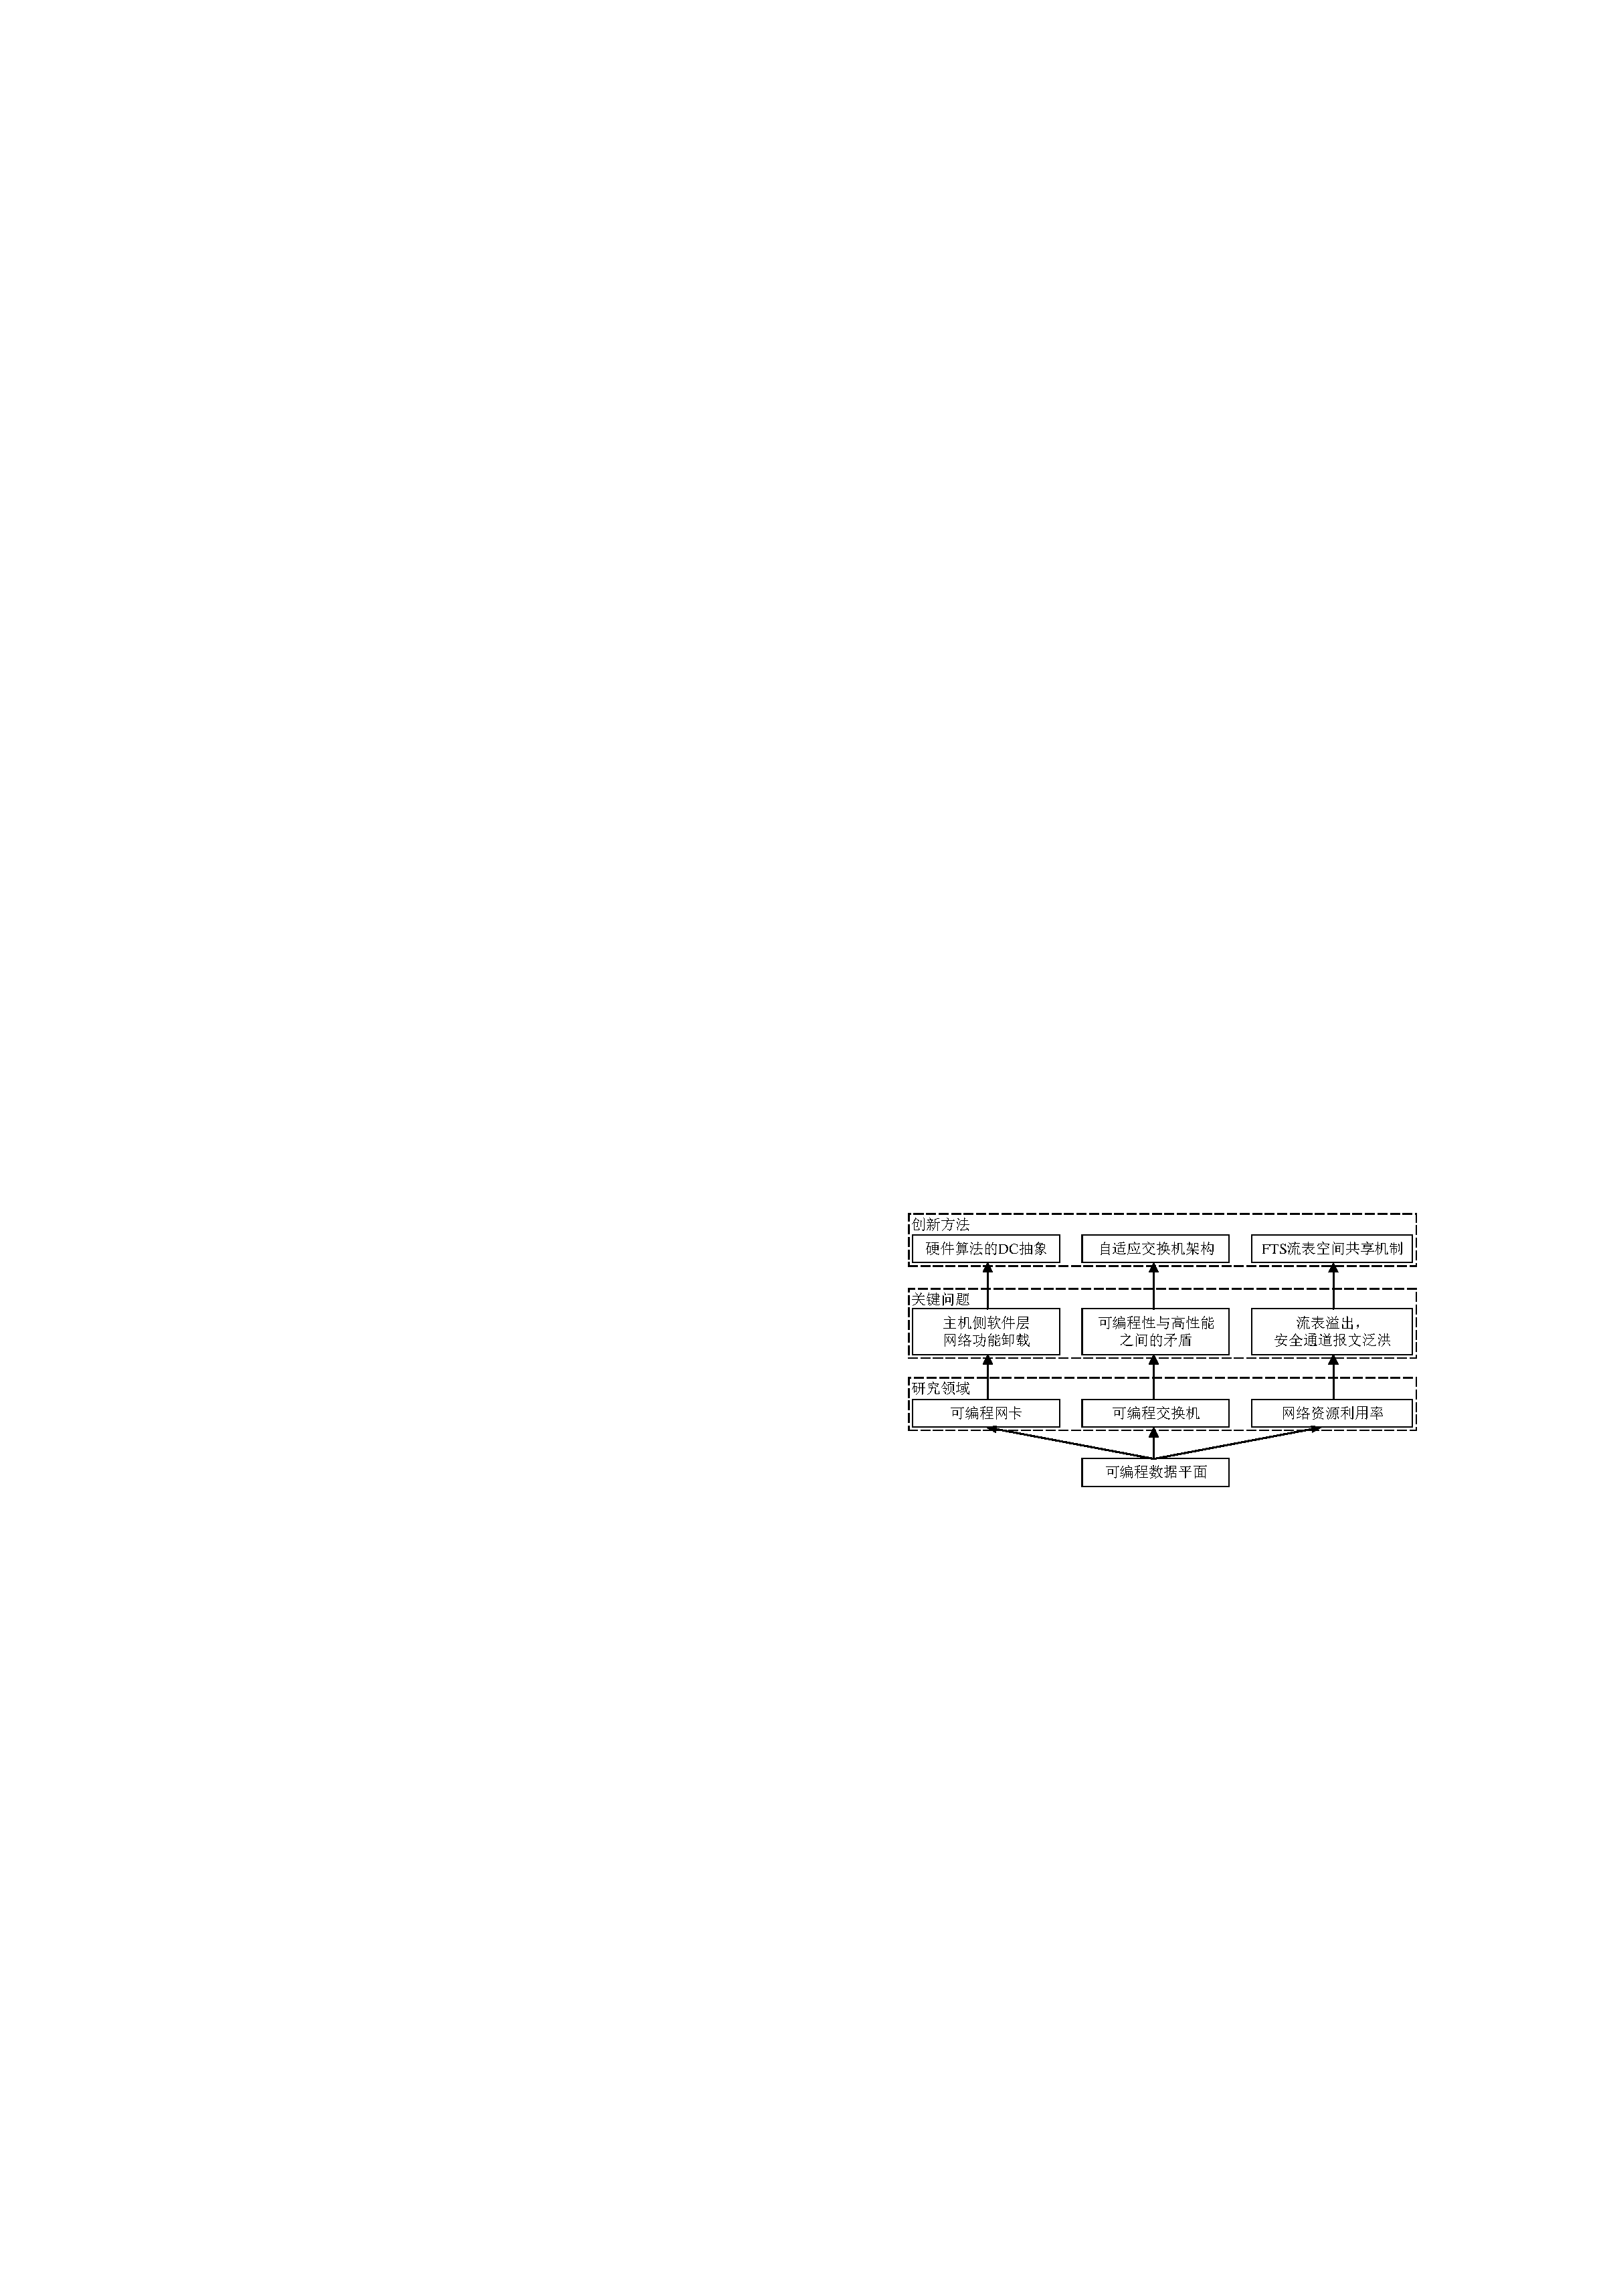
\includegraphics[scale=1]{thesistree.pdf}
	\caption{论文主要研究内容以及成果} \label{thesistree}
\end{figure}

论文针对可编程网卡卸载有状态计算和流量工程、基于FPGA可编程硬件性能不足,流表溢出威胁风险大网络资源利用率低等问题展开分析和创新方法设计。如图\ref{thesistree}具体研究成果概况如下:

1)提出了针对流量随路计算的网络功能卸载抽象模型

本文提出一种适用于网络功能硬件卸载的抽象模型:数据—计算抽象(DATA—COMPUTING, DC抽象)。根据DC抽象,分离软件中适用于硬件加速的繁杂计算,使原本经X86计算架构需要频繁访存的任务,转换到硬件中做流水线式流计算,可在不影响功能精度的前提下,释放CPU资源,大规模扩展性能,提升系统效率。同时,再配合数据包的分类—查找抽象(Classification—Matching,CM抽象),论文在可编程硬件的网卡中实现了更高精度、更高性能、资源利用率更好的流量捕获-统计-回放应用。在满足网络功能不受影响的前提下,证明利用可编程硬件能使原有软件性能效提升100x、抖动降低4次方数量级、能源效率提升10x。

%(统计里介绍存储,看《阿里巴巴》240页的内存类型。后面大叙述里使用)
2)提出了FPGA与交换芯片(Switching ASIC)结合的自适应交换机架构

本文提出一种高性能的可重配交换层数据平面架构:自适应交换结构(Adaptive Switch, AS)。通过FPGA与交换芯片联合的设计思想,AS架构将FPGA的高灵活性与交换芯片的强大性能同时对外表现。论文在前述DC抽象的基础上,继续研究FPGA可编程硬件中高度并行的大规模性能扩展方法。为了保证FPGA低资源消耗,论文设计了一种基于硬件的灵活负载均衡机制。综上,AS架构解决了FPGA性能差与资源少的限制,与交换芯片的有机连接更进一步增强了AS架构的整体性能。综上在可编程性与纯粹FPGA等同的条件下,论文将目前基于FPGA的可编程数据平面性能提升120x。

%(其实跟自动驾驶网络的背景也能融合)

3)提出了一种针对流表资源不足场景下的网络内流表共享机制

网络转发层核心资源不足的问题,本文提出一种全局流表共享方法(Flow Table Sharing, FTS)。本文分析目前OpenFlow协议中有关Table-Miss(流表缺失)的处理过程,并论证即使单纯依靠增加流表容量的资源堆叠方案,并不能使流表溢出的概率降低为零。本文在维持SDN网络控制面悬离特性不变的前提下,提出新的Table-Miss处理机制。FTS方法通过控制器层面、交换机数据层面的软硬件联合设计方法,使得新的Table-Miss机制能实现对原先受影响的转发流量RTT时间和安全通道消息风暴数量的优化均达到至少2个数量级,并且能够容易回退、向下兼容现阶段的传统方案。


\BiSection{论文组织结构}{arc}

根据主要研究内容的讨论,本文的组织结构安排如下:

第2章 对相关工作进行调研,主要介绍网络中主要数据平面,以及其可编程化发展趋势,分析应对网络软件定义化的主要挑战。

第3章 网络计算、流量工程卸载方法。

第4章 自适应交换机,可编程数据平面,网络交换层。

第5章 网络资源全局优化方法,table-miss处理方法。

第6章 总结。









































%-----------------------------------------------------------------------------------------
%\BiSection{为什么用 \LaTeX}{Why}
%
%虽然论文排版是一项基本技能,但是从实际情况看,同学们经常被各种格式整得晕头转向。加之 Word 排版不够美观,版本管理麻烦,排版效率低下,因此开发 \LaTeX{} 论文模板非常重要。国际上许多著名的出版机构和学术期刊都有自己的 \LaTeX{} 模板,国内外许多高效也有自己的硕博论文 \LaTeX{} 模板。事实上,\LaTeX{} 已经成为科技出版行业的国际标准,特别是数学、物理、计算机和电子信息学科。
%
%采用 \LaTeX{} 排版主要有以下优点:
%\begin{enumerate}
%	\item 排版质量高:主要体现在对版面尺寸的严格控制,对字距、行距和段距等间距的松紧适度掌握,对数学公式的精细设计,对插图和表格的灵活处理,对代码和算法的优美呈现,等等。
%	\item 安全稳定:自发布以来 \TeX{} 和 \LaTeX{} 没有发现系统漏洞,不会出现死机或者系统崩溃而导致编写的内容来不及保存。
%	\item 灵活方便:\LaTeX{} 的源文件是纯文本文件,文件大小比 Word 小很多,不会因为文容的增加而导致文档打开、编辑、保存和关闭等操作变慢。因为 \LaTeX{} 在编译时才将所有源文件和图表汇总,故撰写内容时可以随意增删章节和图表。并且和大部分程序设计语言一样,\LaTeX{} 具有注释功能,作者可以在源文件任何地方添加注释,而不会影响最终生成的文档。
%	\item 格式和内容分离:\LaTeX{} 将文档格式和文档内容分开处理,作者只要选择合适的模板,就可专心致志地撰写文档内容,文档的格式细节则由 \LaTeX{} 模板统一规划设置。特别是文献管理能力非常强大,这给撰写像博士论文一样需要大量引用参考文献的文档提供了很大便利。
%	\item 免费开源:\LaTeX{} 软件完全免费,源代码也全部公开,并且相应的配套软件也都采用开源的方式。
%\end{enumerate}
%
%无论你是因为羡慕 \LaTeX{} 漂亮的输出结果,还是因为要给学术期刊投稿而被逼上梁山,都不得不面对这样一个事实:\LaTeX{} 是一种并不简单的排版软件,不可能只点点鼠标就弄好一篇漂亮的文章。还得拿出点搞研究的精神,通过不断练习,才能编排出整齐漂亮的论文。一旦你掌握了如何使用 \LaTeX{} 撰写出精美漂亮的论文时,你会发现你的决定是明智的,你的投入是值得的。
%
%%=========================================================================================
%\BiSection{怎样用 \LaTeX}{How} 
%
%本模板在 Windows + TeXLive2016 + Texsdudio 平台下开发,采用 XeLaTex 编译。虽然之前也开发过一个基于 CTeX 的模板,但是经过多方面比较发现 TeXLive+XeLaTex 处理中文更好,所以基于 CTeX 的模板没有共享。
%
%{\color{red}本模板不能在 CTeX 软件下使用,必须采用 TeXLive,并且编译方式是 XeLaTeX。TeXLive 每年更新一个版本,我用的是 TeXLive2016。文本编辑器可以根据自己的喜好选用,我用的是 Texsdudio,这款开源软件非常不错,推荐大家使用。}
%
%本模板的源文件通过主目录下的 main.tex 统一管理,setup 文件夹中存放格式定义和封面、摘要、目录等内容,body 文件夹中存放论文正文章节的源文件,appendix 文件夹中存放附录、致谢和声明等内容。
%
%本模板只提供论文的格式定义,不提供 \LaTeX{} 的详细使用方法。%所以只回复和论文格式相关的问题,不解答具体的排版方法和技巧。
%因为 \LaTeX{} 的资源非常丰富,大家可以在网上查找资料和并参与讨论,这样学习效率更高。我关注的两个网站是:\url{http://bbs.ctex.org/forum.php} 和 \url{http://www.latexstudio.net};参考的两本书是 ``The Not So Short Introduction to \LaTeXe'' 和 ``LaTeX2e完全学习手册''。
